\documentclass[letterpaper,12pt]{article}
\usepackage[utf8]{inputenc}
\usepackage[top=1.25in, bottom=1.25in, left=1in, right=1in]{geometry}
\usepackage{amsmath}
\usepackage{amsthm}
\usepackage{amsfonts}
\usepackage{enumitem}
\usepackage{hyperref}
\usepackage{subcaption}
\usepackage{graphicx}

\setenumerate{parsep=0em, listparindent=\parindent}

\DeclareMathOperator{\Tr}{Tr}
\DeclareMathOperator{\dom}{dom}
\DeclareMathOperator{\diag}{diag}
\DeclareMathOperator{\dist}{dist}
\DeclareMathOperator{\spn}{span}
\DeclareMathOperator{\prob}{P}
\DeclareMathOperator{\E}{E}
\DeclareMathOperator{\conv}{conv}
\DeclareMathOperator*{\argmax}{arg\,max}
\DeclareMathOperator*{\argmin}{arg\,min}

%\newcommand{\norm}[1]{\left\lVert#1\right\rVert}
\newcommand{\norm}[1]{\lVert#1\rVert}
\newcommand{\ceil}[1]{\left\lceil#1\right\rceil}
\newcommand{\floor}[1]{\left\lfloor#1\right\rfloor}

\newtheorem{innercustomgeneric}{\customgenericname}
\providecommand{\customgenericname}{}
\newcommand{\newcustomtheorem}[2]{%
  \newenvironment{#1}[1]
  {%
   \renewcommand\customgenericname{#2}%
   \renewcommand\theinnercustomgeneric{##1}%
   \innercustomgeneric
  }
  {\endinnercustomgeneric}
}

\newcustomtheorem{customthm}{Theorem}
\newcustomtheorem{customlemma}{Lemma}

\newtheorem{theorem}{Theorem}

\title{Final Project: Signed Support Recovery with the LASSO}
\author{Benjamin Noland}
\date{}

\begin{document}

\maketitle

\section*{Introduction}

A common problem in applied statistics is estimation of a vector
$\beta^\ast \in \mathbb{R}^p$ of unknown but fixed parameters in the
linear model
\begin{equation} \label{eq:linear_model}
  y = X\beta^\ast + \epsilon,
\end{equation}
where $y \in \mathbb{R}^n$ is a vector of observed responses,
$X \in \mathbb{R}^{n \times p}$ is the design matrix, and
$\epsilon \in \mathbb{R}^n$ is a zero-mean random vector representing
the uncertainty in the model.

In the classical setting, we assume that the number of parameters $p$
is small relative to the number of observations, specifically
$p \leq n$. In this setting, assuming the design matrix $X$ has full
row rank, straightforward linear algebra yields an explicit, unique
least-squares estimator of $\beta^\ast$.

However, the situation when there are more parameters than
observations, i.e., $p > n$, is not so well understood, and belongs to
the active area of research known as \textit{high-dimensional
  statistics}. One of the strategies commonly employed in
high-dimensional statistics is to assume that the data is \emph{truly
  low-dimensional} in some sense. In the context of our linear model
\eqref{eq:linear_model}, this means assuming that a large number of
the entries of the true parameter vector $\beta^\ast$ are zero. To be
precise, define the \textit{support} of $\beta^\ast$ by
\begin{equation*}
  S(\beta^\ast) = \{i \in \{1, \ldots, p\} : \beta^\ast_i \neq 0\},
\end{equation*}
and let $k = |S(\beta^\ast)|$ denote its cardinality, i.e., the number
of non-zero entries of $\beta^\ast$. We assume that the vector
$\beta^\ast$ is \textit{sparse}, in the sense that $k \ll p$. Under
this \textit{sparsity assumption}, the problem reduces to that of
computing the support $S(\beta^\ast)$, allowing us to identify which
parameters in the vector $\beta^\ast$ are truly important. In this
way, we have the potential to substantially reduce the dimensionality
of the original problem.

A computationally tractable method for computing estimates of the
parameters $\beta^\ast$ in the high-dimensional setting is the
\textit{LASSO} \cite{tibshirani96} (Least Absolute Shrinkage And
Selection Operator). The LASSO computes an estimate of $\beta^\ast$ as
a solution $\hat{\beta} \in \mathbb{R}^p$ to the following
$l_1$-constrained quadratic program:
\begin{equation} \label{eq:constrained_problem}
  \begin{array}{ll}
    \text{minimize} & \norm{y - X\beta}_2^2 \\
    \text{subject to}
      & \norm{\beta}_1 \leq C_n
  \end{array},
\end{equation}
where $C_n > 0$, or equivalently, as the solution to the unconstrained
problem
\begin{equation} \label{eq:unconstrained_problem}
  \text{minimize} \
    \frac{1}{2n} \norm{y - X\beta}_2^2 + \lambda_n \norm{\beta}_1,
\end{equation}
where $\lambda_n \geq 0$ is a \textit{regularization parameter} that
is in one-to-one correspondence with $C_n$ via Lagrangian duality
\cite{wainwright06}.

\section*{Project overview}

This project will explore the contributions of the paper
\cite{wainwright06} to the problem of inferring the support
$S(\beta^\ast)$ of $\beta^\ast$ (i.e., the problem of \textit{support
  recovery}) in the linear model \eqref{eq:linear_model} using the
LASSO as a means of estimating $\beta^\ast$, as well as consider the
effects of altering the LASSO $l_1$-penalty on support recovery.

\subsection*{Overview of the paper}

The paper \cite{wainwright06} provides both necessary and sufficient
conditions for the LASSO to recover the \textit{signed support}
$\mathbb{S}_\pm(\beta^\ast) \in \mathbb{R}^p$ of $\beta^\ast$ with
high probability, where $\mathbb{S}_\pm(\beta)$ is defined as follows
for any $\beta \in \mathbb{R}^p$:
\begin{equation*}
  \mathbb{S}_\pm(\beta)_i =
  \begin{cases}
    +1 & \quad \text{if $\beta_i > 0$} \\
    -1 & \quad \text{if $\beta_i < 0$} \\
    0 & \quad \text{if $\beta_i = 0$}
  \end{cases}
  \quad (i = 1, \ldots, p).
\end{equation*}
Specifically, the authors consider the following two questions:
\begin{itemize}
\item What relationships between $n$, $p$, and $k$ yield a
  \emph{unique} LASSO solution $\hat{\beta} \in \mathbb{R}^p$
  satisfying
  $\mathbb{S}_\pm(\hat{\beta}) = \mathbb{S}_\pm(\beta^\ast)$?
\item For what relationships between $n$, $p$, and $k$ does \emph{no
    solution} of the LASSO yield the correct signed support?
\end{itemize}
These questions are analyzed for both deterministic designs and random
designs in the linear model \eqref{eq:linear_model}.

In addition to providing theoretical guarantees, the authors describe
the results of simulations to investigate the success/failure of the
LASSO in recovering the true signed support for random designs under
each of the following sparsity regimes:
\begin{itemize}
\item \textit{linear sparsity}: $k(p) = \ceil{\gamma p}$ for some
  $\gamma \in (0, 1)$;
\item \textit{sublinear sparsity}:
  $k(p) = \ceil{\gamma p / \log(\gamma p)}$ for some
  $\gamma \in (0, 1)$, and
\item \textit{fractional power sparsity}:
  $k(p) = \ceil{\gamma p^\delta}$ for some
  $\gamma, \delta \in (0, 1)$.
\end{itemize}
In each case, the authors take $\gamma = 0.40$ and $\delta = 0.75$,
and the number of observations $n$ is taken to be proportional to
$k\log(p - k)$. The true support of the parameter vector is chosen
uniformly at random subject to the chosen sparsity regime.

For each sparsity regime and for several values of $p$, the authors
compute a sequence of values of the \textit{rescaled sample size} (or
\textit{control parameter}) $\theta = n / (2k \log(p -k))$ and for
each such value, compute a sequence of corresponding LASSO solutions
$\hat{\beta} \in \mathbb{R}^p$ in order to approximate the probability
$\prob\{\mathbb{S}_\pm(\hat{\beta}) = \mathbb{S}_\pm(\beta^\ast)\}$ of
recovering the true signed support. This approximated probability is
then plotted against the control parameter $\theta$.

The first round of experiments samples the design matrix
$X \in \mathbb{R}^{n \times p}$ from a uniform Gaussian ensemble; that
is, its rows are sampled independently from the distribution
$N_p(0, I_p)$. A second round of experiments samples $X$ from a
non-uniform Gaussian ensemble; specifically, one such that the rows
are sampled independently from the distribution $N_p(0, \Sigma)$,
where $\Sigma$ is a $p \times p$ Toeplitz matrix of the form
\begin{equation} \label{eq:toeplitz_covariance}
  \Sigma =
  \begin{pmatrix}
    1 & \mu & \mu^2 & \cdots & \mu^{p-2} & \mu^{p-1} \\
    \mu & 1 & \mu & \mu^2 & \cdots & \mu^{p-2} \\
    \mu^2 & \mu & 1 & \mu & \cdots & \mu^{p-3} \\
    \vdots & \vdots & \vdots & \vdots & \vdots & \vdots \\
    \mu^{p-1} & \cdots & \mu^3 & \mu^2 & \mu & 1
  \end{pmatrix},
\end{equation}
where $\mu = 0.10$. In both cases, the authors note good agreement
with their theoretical predictions.

\subsection*{This project}

In addition to duplicating the simulations from the paper
\cite{wainwright06}, this project extends the simulations by
considering the more general case of \textit{elastic net} penalties
\cite{zou_hastie05}, which extend the $l_1$ penalty in
\eqref{eq:unconstrained_problem} to include an $l_2$ term as
well. Specifically, we consider solutions
$\hat{\beta} \in \mathbb{R}^p$ to the problem
\begin{equation} \label{eq:elastic_net_problem}
  \text{minimize} \
    \frac{1}{2n} \norm{y - X\beta}_2^2
      + \lambda_n \left( \frac{1}{2} (1 - \alpha) \norm{\beta}_2^2
      + \alpha \norm{\beta}_1 \right ),
\end{equation}
where $\lambda_n \geq 0$, and $\alpha \in [0, 1]$ is the elastic net
\textit{mixing parameter}. We repeat the simulations described in
\cite{wainwright06} for the case of uniform Gaussian ensembles, but
instead use elastic net solutions $\hat{\beta} \in \mathbb{R}^p$ for
each of $\alpha = 0.75$ and $\alpha = 0.50$ to estimate the
probability of signed support recovery. We compare the results to
those from the original simulations.

\section*{Theoretical results}

Before describing the simulations in detail, we need to detail their
theoretical basis. We first demonstrate the equivalence of the
$l_1$-constrained QP \eqref{eq:constrained_problem} and the
unconstrained problem \eqref{eq:unconstrained_problem}, the latter of
which is the formulation used directly in the simulations. We then
provide the results from \cite{wainwright06} that give necessary and
sufficient conditions for signed support recovery using the LASSO.

\subsection*{Equivalence of constrained and unconstrained problems}

As noted in the introduction, the $l_1$-constrained problem
\eqref{eq:constrained_problem} is equivalent to the unconstrained
problem \eqref{eq:unconstrained_problem} in the following sense: for
every value of $C_n > 0$ in \eqref{eq:constrained_problem} there
exists a value $\lambda_n \geq 0$ in \eqref{eq:unconstrained_problem}
such that \eqref{eq:unconstrained_problem} is equivalent to
\eqref{eq:constrained_problem}, and vice versa (in fact, it can be
shown that $C_n$ and $\lambda_n$ are in one-to-one
correspondence\footnote{Although this fact will not be proven
  here.}). We now demonstrate this equivalence.

First, we need a lemma. We need to show that the constraint
\begin{equation} \label{eq:l1_constraint}
  \norm{\beta}_1 \leq C_n
\end{equation}
in \eqref{eq:constrained_problem} is equivalent to a finite collection
of linear equality and inequality constraints on $\beta$. We can
assume without loss of generality that $C_n = 1$. Consider the
$l_1$-ball $B = \{\beta \in \mathbb{R}^p : \norm{\beta}_1 \leq
1\}$. Let $\{e_1, \ldots, e_p\}$ denote the standard ordered basis for
$\mathbb{R}^p$. We claim that $B = \conv S$, where
\begin{equation*}
  S = \conv\{e_1, \ldots, e_p, -e_1, \ldots, -e_p\}.
\end{equation*}
If we can show that $B = \conv S$, then $B$ is a polyhedron, so that
the constraint \eqref{eq:l1_constraint} is equivalent to a finite
collection of linear equalities and inequalities.

Note that $S \subseteq B$, and since $B$ is a convex set, and
$\conv S$ is the smallest convex set containing $S$, we have
$\conv S \subseteq B$. Conversely, let $\beta \in B$. Then there exist
$a_1, \ldots, a_p \in \mathbb{R}$ with $\beta = \sum_{i=1}^p a_i
e_i$. Assume without loss of generality that $a_1, \ldots, a_m \geq 0$
and $a_{m+1}, \ldots, a_p < 0$. Then we can write
\begin{align*}
  \beta &= \sum_{i=1}^p a_i e_i \\
    &= \sum_{i=1}^m a_i e_i
      + \sum_{i=m+1}^p (-a_i)(-e_i) \\
    &= \sum_{i=1}^m |a_i| e_i
      + \sum_{i=m+1}^p |a_i| (-e_i).
\end{align*}
Then the coefficients $|a_i| \geq 0$ for every $1 \leq i \leq p$, and
since $\norm{\beta}_1 \leq 1$, we have
\begin{equation*}
  \sum_{i=1}^p |a_i| = \norm{\beta}_1 \leq 1.
\end{equation*}
Now, $0 \in \conv S$ since we can write
$0 = (1/2) e_1 + (1/2) (-e_1)$. Therefore,
\begin{equation*}
  \beta = \sum_{i=1}^m |a_i| e_i + \sum_{i=m+1}^p |a_i| (-e_i)
    + (1 - \norm{\beta}_1) \cdot 0 \in \conv S.
\end{equation*}
This shows that $B \subseteq \conv S$, and therefore $B = \conv S$.

Now for the main argument. Let $\hat{\beta} \in \mathbb{R}^p$ be a
solution to the constrained problem
\eqref{eq:constrained_problem}. The Lagrangian of this problem is
\begin{equation*}
  L(\beta, \lambda) = \frac{1}{2n} \norm{y - X\beta}_2^2
    + \lambda(\norm{\beta}_1 - C_n),
\end{equation*}
where $\lambda \in \mathbb{R}$, and so the Lagrange dual function is
given by
\begin{equation*}
  g(\lambda) = \inf_{\beta \in \mathbb{R}^p} L(\beta, \lambda)
    = \inf_{\beta \in \mathbb{R}^p} \left [ \frac{1}{2n} \norm{y - X\beta}_2^2
      + \lambda(\norm{\beta}_1 - C_n) \right ].
\end{equation*}
Note that for any $\lambda \geq 0$, $g(\lambda) > -\infty$, so that
the dual problem
\begin{equation} \label{eq:dual_problem}
  \begin{array}{ll}
    \text{maximize} & g(\lambda) \\
    \text{subject to}
      & \lambda \geq 0
  \end{array}
\end{equation}
is always feasible. Now, since $\hat{\beta}$ is a solution to the
primal problem \eqref{eq:constrained_problem}, it in particular
satisfies $\norm{\beta}_1 \leq C_n$ (i.e., $\hat{\beta}$ is feasible
for the primal problem). By the lemma above, this $l_1$-constraint is
equivalent to a finite number of linear equality and inequality
constraints. Thus Slater's condition is satisfied for
\eqref{eq:constrained_problem}, so that strong duality holds. Since
this problem is convex and its dual problem \eqref{eq:dual_problem} is
feasible, this also implies the existence of a dual solution
$\lambda_n \geq 0$. We therefore conclude that
\begin{align*}
  \hat{\beta} &= \argmin_{\beta \in \mathbb{R}^p} L(\beta, \lambda_n) \\
    &= \argmin_{\beta \in \mathbb{R}^p} \left [ \frac{1}{2n}
      \norm{y - X\beta}_2^2 + \lambda_n (\norm{\beta}_1 - C_n) \right ] \\
    &= \argmin_{\beta \in \mathbb{R}^p} \left [ \frac{1}{2n}
      \norm{y - X\beta}_2^2 + \lambda_n \norm{\beta}_1 \right ],
\end{align*}
i.e., $\hat{\beta}$ is a solution to the unconstrained problem
\eqref{eq:unconstrained_problem}.

Conversely, let $\hat{\beta} \in \mathbb{R}^p$ be a solution to the
unconstrained problem \eqref{eq:unconstrained_problem}. We claim that
$\hat{\beta}$ is a solution to the constrained problem
\eqref{eq:constrained_problem} with $C_n =
\norm{\hat{\beta}}_1$. First, note that $\hat{\beta}$ is clearly
feasible due to the choice of $C_n$. Suppose it is \emph{not} optimal,
i.e., there exists a feasible point $\tilde{\beta} \in \mathbb{R}^p$
with
\begin{equation*}
  \frac{1}{2n} \norm{y - X\tilde{\beta}}_2^2
    < \frac{1}{2n} \norm{y - X\hat{\beta}}_2^2.
\end{equation*}
Since $\tilde{\beta}$ is feasible,
$\norm{\tilde{\beta}}_1 \leq C_n = \norm{\hat{\beta}}_1$. Thus,
\begin{equation*}
  \frac{1}{2n} \norm{y - X\tilde{\beta}}_2^2 + \lambda_n \norm{\tilde{\beta}}_1
    < \frac{1}{2n} \norm{y - X\hat{\beta}}_2^2
      + \lambda_n \norm{\tilde{\beta}}_1
    \leq \frac{1}{2n} \norm{y - X\hat{\beta}}_2^2
      + \lambda_n \norm{\hat{\beta}}_1,
\end{equation*}
contradicting the assumption that $\hat{\beta}$ was optimal for
\eqref{eq:unconstrained_problem}. Hence $\hat{\beta}$ is a solution to
\eqref{eq:constrained_problem} with this choice of $C_n$.

\subsection*{Conditions for signed support recovery}

The paper \cite{wainwright06} provides necessary and sufficient
conditions for the LASSO to recover the signed support of the true
parameter $\beta^\ast$ in the model \eqref{eq:linear_model} for both
deterministic and random designs. Here we restrict our attention to
the case of random design, and state the pertinent results from
\cite{wainwright06}.

The design matrix $X \in \mathbb{R}^{n \times p}$ is in this case
drawn from a random Gaussian ensemble; that is, its rows are sampled
independently from the distribution $N_p(0, \Sigma)$ for some choice
of covariance matrix $\Sigma$.

First, some notation. Let $S = S(\beta^\ast)$ denote the true support
set. For any subset $A \subseteq \{1, 2, \ldots, p\}$, let $X_A$
denote the $n \times |A|$ matrix formed by concatenating the columns
$\{X_i : i \in A\}$ indexed by $A$. When applied to matrices $M$, the
notation $\norm{M}_\infty$ denotes the norm defined by
$\norm{M}_\infty = \max_i \sum_j |M_{ij}|$; when applied to vectors,
it denotes the usual $l_\infty$-norm. The symbols $c_1, c_2$,
etc. denote positive constants whose values may differ from line to
line.

The results given below rely upon (subsets of) the following
conditions on $\Sigma$ being satisfied:
\begin{subequations}
  \begin{align}
    \norm{\Sigma_{S^c S} \Sigma_{SS}^{-1}}_\infty &\leq 1 - \gamma
      \quad \text{for some $\gamma \in (0, 1]$}
      \label{eq:cov_cond_a} \\
    \Lambda_{\mathrm{min}}(\Sigma_{SS}) &\geq C_{\mathrm{min}} > 0
      \label{eq:cov_cond_b} \\
    \Lambda_{\mathrm{max}}(\Sigma_{SS}) &\leq C_{\mathrm{max}} < \infty,
      \label{eq:cov_cond_c}
  \end{align}
\end{subequations}
where $\gamma$ is known as an \textit{incoherence parameter}, and
\begin{align*}
  \Sigma_{SS} &= \E \left ( \frac{1}{n} X_S^T X_S \right ) \\
  \Sigma_{S^c S} &= \E \left ( \frac{1}{n} X_{S^c}^T X_S \right ),
\end{align*}
and similarly for $\Sigma_{SS^c}$ and $\Sigma_{S^c S^c}$. The
expressions $\Lambda_{\mathrm{min}}(\Sigma_{SS})$ and
$\Lambda_{\mathrm{max}}(\Sigma_{SS})$ denote the minimum and maximum
eigenvalues of $\Sigma_{SS}$, respectively.

For a positive semidefinite matrix $A$, define
\begin{align*}
  \rho_l(A) &= \frac{1}{2} \min_{i \neq j} (A_{ii} + A_{jj} - 2A_{ij}) \\
  \rho_u(A) &= \max_i A_{ii}.
\end{align*}
It is not difficult to show that
\begin{equation*}
  0 \leq \rho_l(A) \leq \rho_u(A).
\end{equation*}

Finally, using the conditional covariance matrix
\begin{equation*}
  \Sigma_{S^c | S}
    = \Sigma_{S^c S^c} - \Sigma_{S^c S} \Sigma_{SS}^{-1} \Sigma_{SS^c}
    \succeq 0
\end{equation*}
of $(X_{S^c} | X_S)$, we define
\begin{align*}
  \theta_l(\Sigma) &= \frac{\rho_l(\Sigma_{S^c | S})}
    {C_{\mathrm{max}} (2 - \gamma(\Sigma))} \\
  \theta_u(\Sigma) &= \frac{\rho_u(\Sigma_{S^c | S})}
    {C_{\mathrm{min}} \gamma(\Sigma)^2},
\end{align*}
where $\gamma(\Sigma) \in (0, 1]$ is the incoherence parameter in
\eqref{eq:cov_cond_a}. Moreover, we have the inequalities
\begin{equation*}
  0 \leq \theta_l(\Sigma) \leq \theta_u(\Sigma) < \infty.
\end{equation*}

With these definitions and conditions in place, we are now able to
state the pertinent results from \cite{wainwright06}. The first
result, Theorem~\ref{sufficiency} from \cite{wainwright06}, provides
sufficient conditions for the LASSO to recover the signed support of
the true parameter $\beta^\ast$ in the linear model
\eqref{eq:linear_model}.
\begin{customthm}{3}[Sufficiency] \label{sufficiency}

  Consider the linear model \eqref{eq:linear_model} with random
  Gaussian design $X \in \mathbb{R}^{n \times p}$ and error term
  $\epsilon \sim N_n(0, \sigma^2 I_n)$. Assume that the covariance
  matrix $\Sigma$ satisfies conditions \eqref{eq:cov_cond_a} and
  \eqref{eq:cov_cond_b}. Consider the sequence $(\lambda_n)$ of
  regularization parameters given by
  \begin{equation} \label{eq:lambda_sequence}
    \lambda_n = \lambda_n(\phi_p)
      = \sqrt{\frac{\phi_p \rho_u(\Sigma_{S^c|S})}{\gamma^2}
        \frac{2\sigma^2 \log p}{n}},
  \end{equation}
  where $\phi_p \geq 2$. Suppose there exists $\delta > 0$ such that
  the sequences $(n, p, k)$ and $(\lambda_n)$ satisfy
  \begin{equation*}
    \frac{n}{2k \log (p - k)}
      > (1 + \delta) \theta_u(\Sigma)
        \left ( 1 + \frac{\sigma^2 C_{\mathrm{min}}}{\lambda_n^2 k}
        \right ).
  \end{equation*}
  Then the following properties hold with probability
  $> 1 - c_1 \exp(-c_2 \min\{k, \log(p - k)\})$:
  \begin{enumerate}[label=(\roman*)]
  \item The LASSO has a unique solution $\hat{\beta} \in \mathbb{R}^p$
    with $S(\hat{\beta}) \subseteq S(\beta^\ast)$ (i.e., its support
    is contained in the true support).

  \item Define
    \begin{equation*}
      g(\lambda_n) = c_3 \lambda_n \norm{\Sigma_{SS}^{-1/2}}_\infty^2
        + 20\sqrt{\frac{\sigma^2 \log k}{C_{\mathrm{min}} n}}.
    \end{equation*}
    Then if $\beta_{\mathrm{min}} = \min_{i \in S} |\beta^\ast_i|$
    satisfies $\beta_{\mathrm{min}} > g(\lambda_n)$, we have
    \begin{equation*}
      \mathbb{S}_\pm(\hat{\beta}) = \mathbb{S}_\pm(\beta^\ast)
    \end{equation*}
    and
    \begin{equation*}
      \norm{\hat{\beta}_S - \beta^\ast_s}_\infty \leq g(\lambda_n).
    \end{equation*}
  \end{enumerate}
\end{customthm}
The second result, Theorem~\ref{necessity} from \cite{wainwright06}
provides \emph{necessary} conditions for signed support recovery to be
successful. Specifically, it provides sufficient conditions for signed
support recovery to fail. Thus, in order for the LASSO to recover the
true signed support with high probability, the conditions of
Theorem~\ref{necessity} \emph{must not} be satisfied.
\begin{customthm}{4}[Necessity] \label{necessity}

  Consider the linear model \eqref{eq:linear_model} with random
  Gaussian design $X \in \mathbb{R}^{n \times p}$ and error term
  $\epsilon \sim N_n(0, \sigma^2 I_n)$. Assume that the covariance
  matrix $\Sigma$ satisfies conditions \eqref{eq:cov_cond_a},
  \eqref{eq:cov_cond_b}, and \eqref{eq:cov_cond_c}. Consider the
  sequence $(\lambda_n)$ of regularization parameters
  \eqref{eq:lambda_sequence}. Suppose there exists $\delta > 0$ such
  that the sequences $(n, p, k)$ and $(\lambda_n)$ satisfy
  \begin{equation*}
    \frac{n}{2k \log (p - k)}
      < (1 - \delta) \theta_l(\Sigma)
        \left ( 1 + \frac{\sigma^2 C_{\mathrm{max}}}{\lambda_n^2 k}
        \right ).
  \end{equation*}
  Then with probability converging to one, no solution of the LASSO
  has the correct signed support.
\end{customthm}

\section*{Simulations}

We are now prepared to describe the simulations. The first two sets of
simulations duplicate those from \cite{wainwright06}, using LASSO
solutions to calculate the probability of signed support recovery for
a variety of problem sizes $p$ in the following two cases,
respectively:
\begin{enumerate}
\item the design matrix $X$ is drawn from a uniform Gaussian ensemble
  ($\Sigma = I_p$);
\item the design matrix $X$ is drawn from a non-uniform Gaussian
  ensemble where $\Sigma$ is Toeplitz of the form
  \eqref{eq:toeplitz_covariance}.
\end{enumerate}
We consider models fit using the family of regularization parameters
$\lambda_n$ given by
\begin{equation*}
  \lambda_n = \sqrt{\frac{2\sigma^2 \log k \log(p - k)}{n}},
\end{equation*}
where $\sigma = 0.5$ is a fixed noise level. For this choice of
$\lambda_n$, Theorem~\ref{necessity} predicts failure with high
probability for sequences $(n, p, k)$ satisfying
\begin{equation*}
  \frac{n}{2k \log(p - k)} < \theta_l(\Sigma),
\end{equation*}
and Theorem~\ref{sufficiency} predicts success with high probability
for sequences $(n, p, k)$ such that
\begin{equation*}
  \frac{n}{2k \log(p - k)} > \theta_u(\Sigma)
\end{equation*}
(see \cite{wainwright06}). These simulations are conducted for linear,
sublinear, and fractional power sparsity regimes.

The second two sets of simulations are the same as the first set
(uniform Gaussian ensemble), except that the penalty function in the
LASSO objective is generalized to an elastic net penalty. For these
last two simulations we use elastic net mixing parameters
$\alpha = 0.75$ and $\alpha = 0.50$, respectively.

The simulation code was written in R and can be found in the file
\texttt{simulations.R}. The R package
\texttt{glmnet}\footnote{\url{https://cran.r-project.org/web/packages/glmnet/index.html}}
was used to compute LASSO and elastic net solutions.

\subsection*{Methodology}

We fix $\gamma = 0.40$ and $\delta = 0.75$ for computing the sparsity
indices, and fix a noise level $\sigma = 0.5$. For a fixed sparsity
regime, the following is then repeated for each of the problem sizes
$p \in \{128, 256, 512\}$:

\begin{enumerate}
\item We first compute the sparsity index $k$ (under the chosen
  sparsity regime) from the problem size $p$. We then generate a
  support set $S$ of size $p$ and with sparsity index $k$ uniformly at
  random, and use $S$ to generate the true parameter $\beta^\star$
  whose signed support is to be estimated. Specifically, for each
  $i \in S$, we set $\beta^\ast_i = \beta_{\mathrm{min}}$ or
  $\beta^\ast_i = -\beta_{\mathrm{min}}$, where
  $\beta_{\mathrm{min}} = 0.5$, uniformly at random, and set
  $\beta^\ast_i = 0$ for each $i \in S^c$. Thus $\beta^\ast$ has
  support $S$. We then compute the signed support
  $\mathbb{S}_\pm(\beta^\ast)$ of $\beta^\ast$.

\item We compute a sequence of 15 equally-spaced control parameters
  $\theta$ in the range $[0.01, 2.4]$. For each of these values
  $\theta$, we compute the associated sample size
  $n = \ceil{2 \theta k \log(p - k)}$ and regularization parameter
  $\lambda_n$, given by
    \begin{equation*}
      \lambda_n = \sqrt{\frac{2\sigma^2 \log k \log(p - k)}{n}},
    \end{equation*}
    and repeat the following for 200 trials:
  \begin{enumerate}
  \item Sample a design matrix $X \in \mathbb{R}^{n \times p}$ from
    the chosen Gaussian ensemble (uniform or non-uniform).
  \item Sample error terms $\epsilon \sim N_n(0, \sigma^2 I_n)$ and
    compute $y = X\beta^\ast + \epsilon$.
  \item Fit a model (LASSO or elastic net) corresponding to the
    regularization parameter $\lambda_n$ and compare the signed
    support $\mathbb{S}_\pm(\hat{\beta})$ of the estimated parameter
    vector $\hat{\beta} \in \mathbb{R}^p$ to the signed support
    $\mathbb{S}_\pm(\beta^\ast)$ of the true parameter. We keep track
    of the number of times the model recovered the correct signed
    support.
  \end{enumerate}
  Finally, we use the results of these 200 trials to compute an
  estimate of the probability
  $\prob\{\mathbb{S}_\pm(\hat{\beta}) = \mathbb{S}_\pm(\beta^\ast)\}$
  of recovering the true signed support.

\item We then plot the values of the control parameter $\theta$
  against our corresponding estimates of
  $\prob\{\mathbb{S}_\pm(\hat{\beta}) =
  \mathbb{S}_\pm(\beta^\ast)\}$. The results for each of the problem
  sizes $p \in \{128, 256, 512\}$ are overlaid on the same graph.
\end{enumerate}

\subsection*{Simulations from the paper}

The first set of simulations from the paper considers signed support
recovery when the design $X \in \mathbb{R}^{n \times p}$ is drawn from
a uniform Gaussian ensemble. In this case, we have $\Sigma = I_p$, and
$\theta_l(I_p) = \theta_u(I_p) = 1$ (see \cite{wainwright06}). Thus we
expect the LASSO to fail to recover the true signed support with high
probability for values of the control parameter
\begin{equation*}
  \theta = \frac{n}{2k \log(p - k)}
\end{equation*}
satisfying $\theta < 1$, and to successfully recover the true signed
support with high probability for values $\theta > 1$. Indeed, the
simulations demonstrate this behavior for each of the three sparsity
regimes in question (see Figure~\ref{fig:uniform_alpha_1}). For
$\theta < 1$, the probability of success is considerably less than 1,
while the probability approaches 1 very quickly for $\theta > 1$. The
behavior for $\theta > 1$ is particularly pronounced for the largest
problem size, $p = 512$.

\begin{figure}[h]
  \centering
  \begin{subfigure}{0.32\textwidth}
    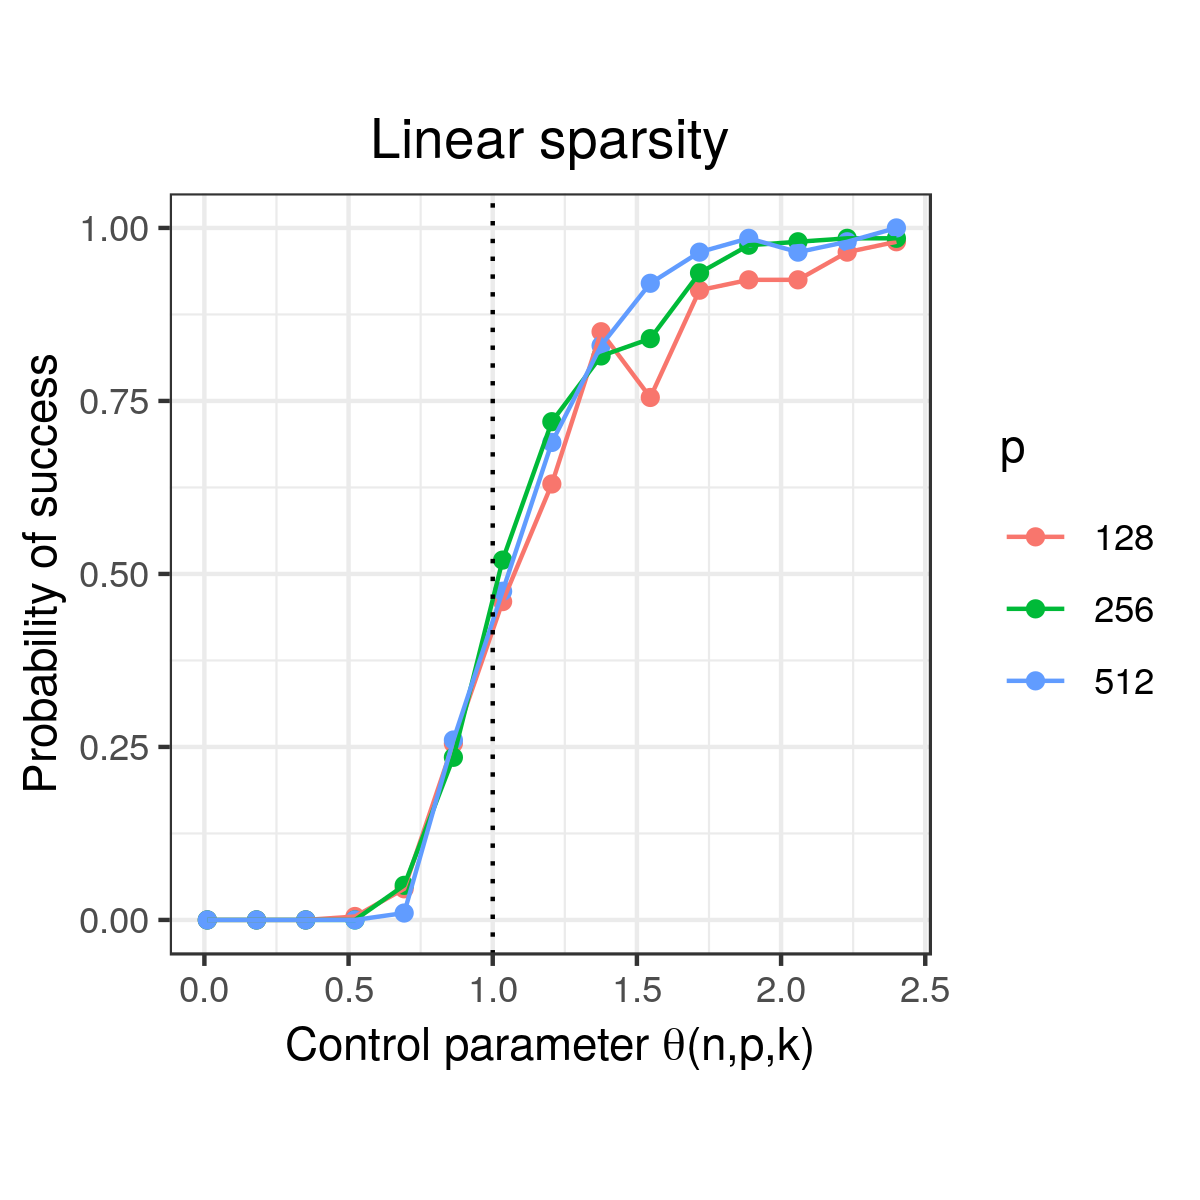
\includegraphics[width=0.9\linewidth]{uniform_linear_sparsity_alpha_1}
    \caption{Linear sparsity}
    \label{fig:uniform_linear_sparsity_alpha_1}
  \end{subfigure}
  \begin{subfigure}{0.32\textwidth}
    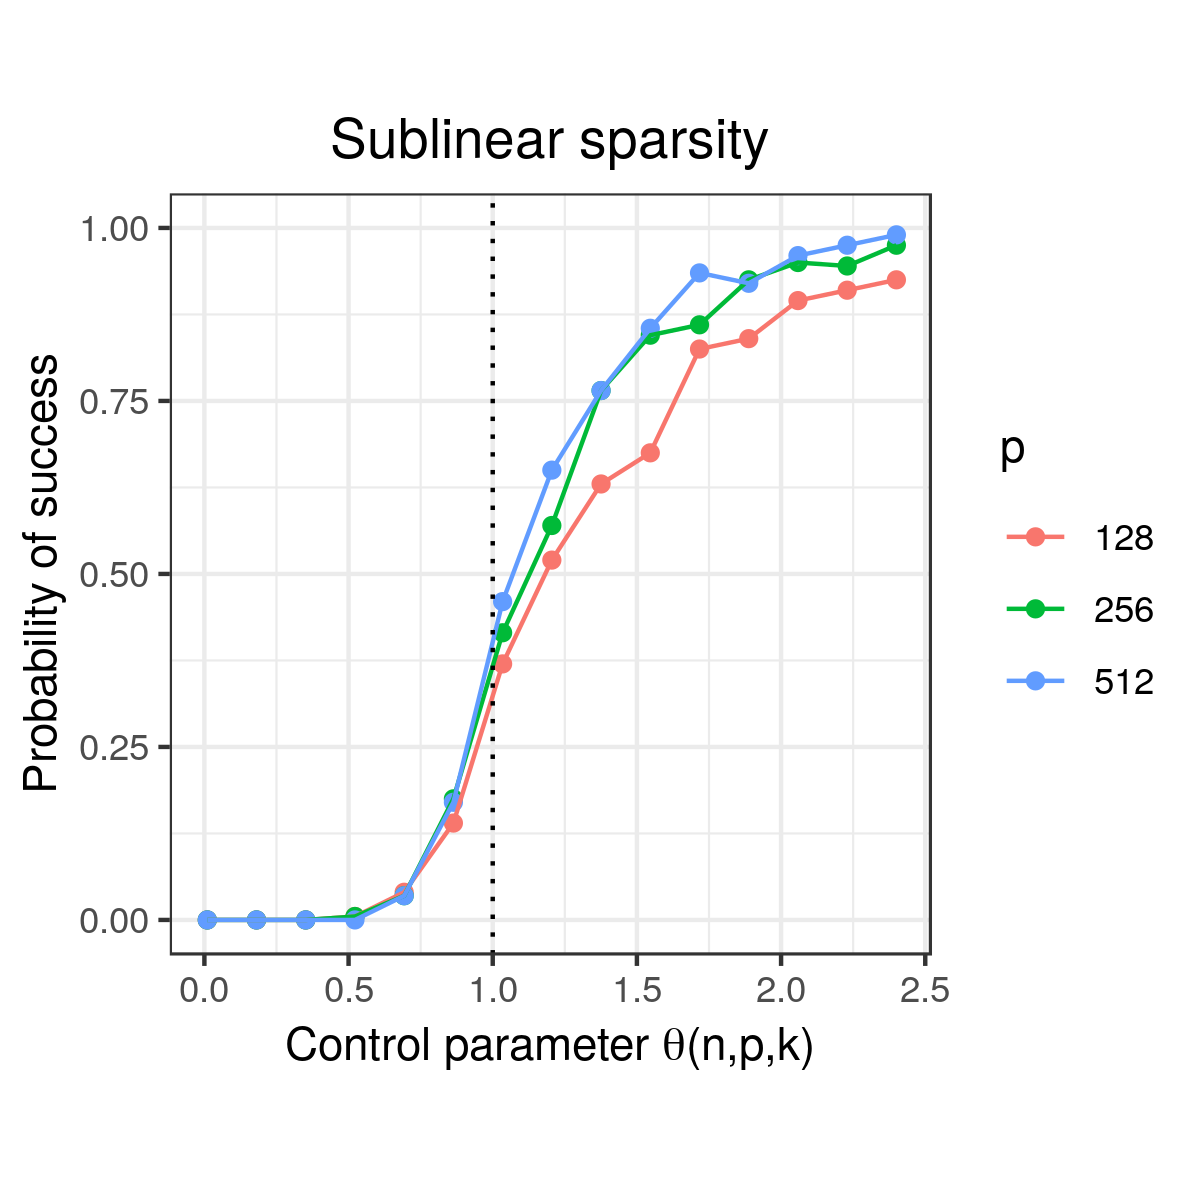
\includegraphics[width=0.9\linewidth]{uniform_sublinear_sparsity_alpha_1}
    \caption{Sublinear sparsity}
    \label{fig:uniform_sublinear_sparsity_alpha_1}
  \end{subfigure}
  \begin{subfigure}{0.32\textwidth}
    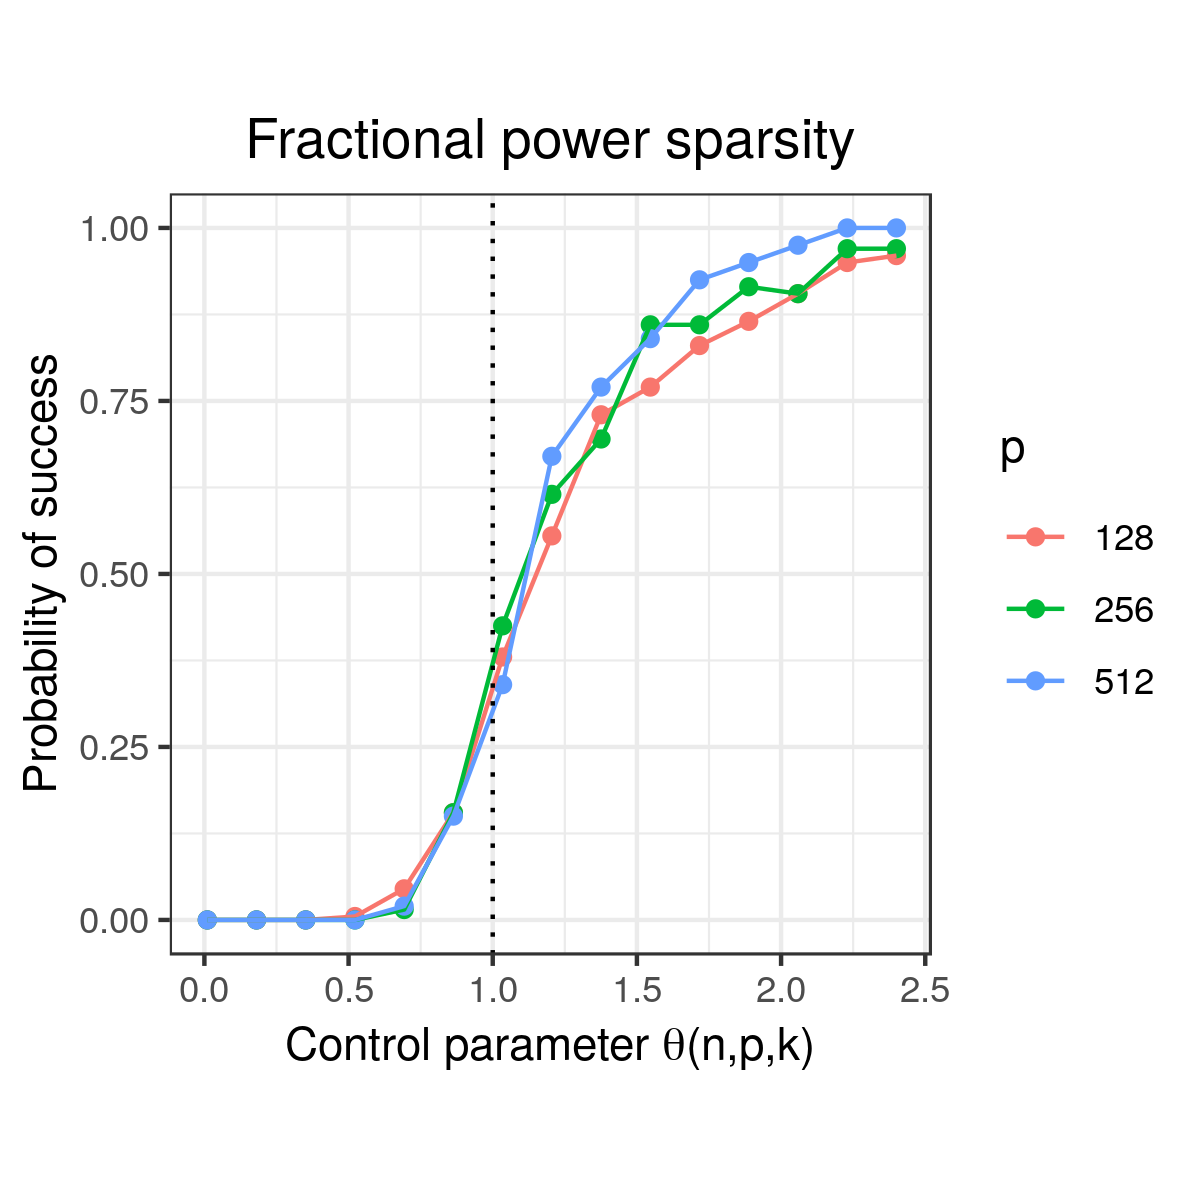
\includegraphics[width=0.9\linewidth]{uniform_fractional_power_sparsity_alpha_1}
    \caption{Fractional power sparsity}
    \label{fig:uniform_fractional_power_sparsity_alpha_1}
  \end{subfigure}
  \caption{Uniform Gaussian ensemble with LASSO}
  \label{fig:uniform_alpha_1}
\end{figure}

The results of the second simulation are similar. In this case the
design matrices are drawn from a non-uniform Gaussian ensemble with
covariance matrix $\Sigma$ of the form \eqref{eq:toeplitz_covariance},
and we have $\theta_l(\Sigma) \approx 1$ and
$\theta_u(\Sigma) \approx 1$ (see \cite{wainwright06}). The results of
this set of simulations are given in
Figure~\ref{fig:nonuniform_alpha_1}.

\begin{figure}[h]
  \centering
  \begin{subfigure}{0.32\textwidth}
    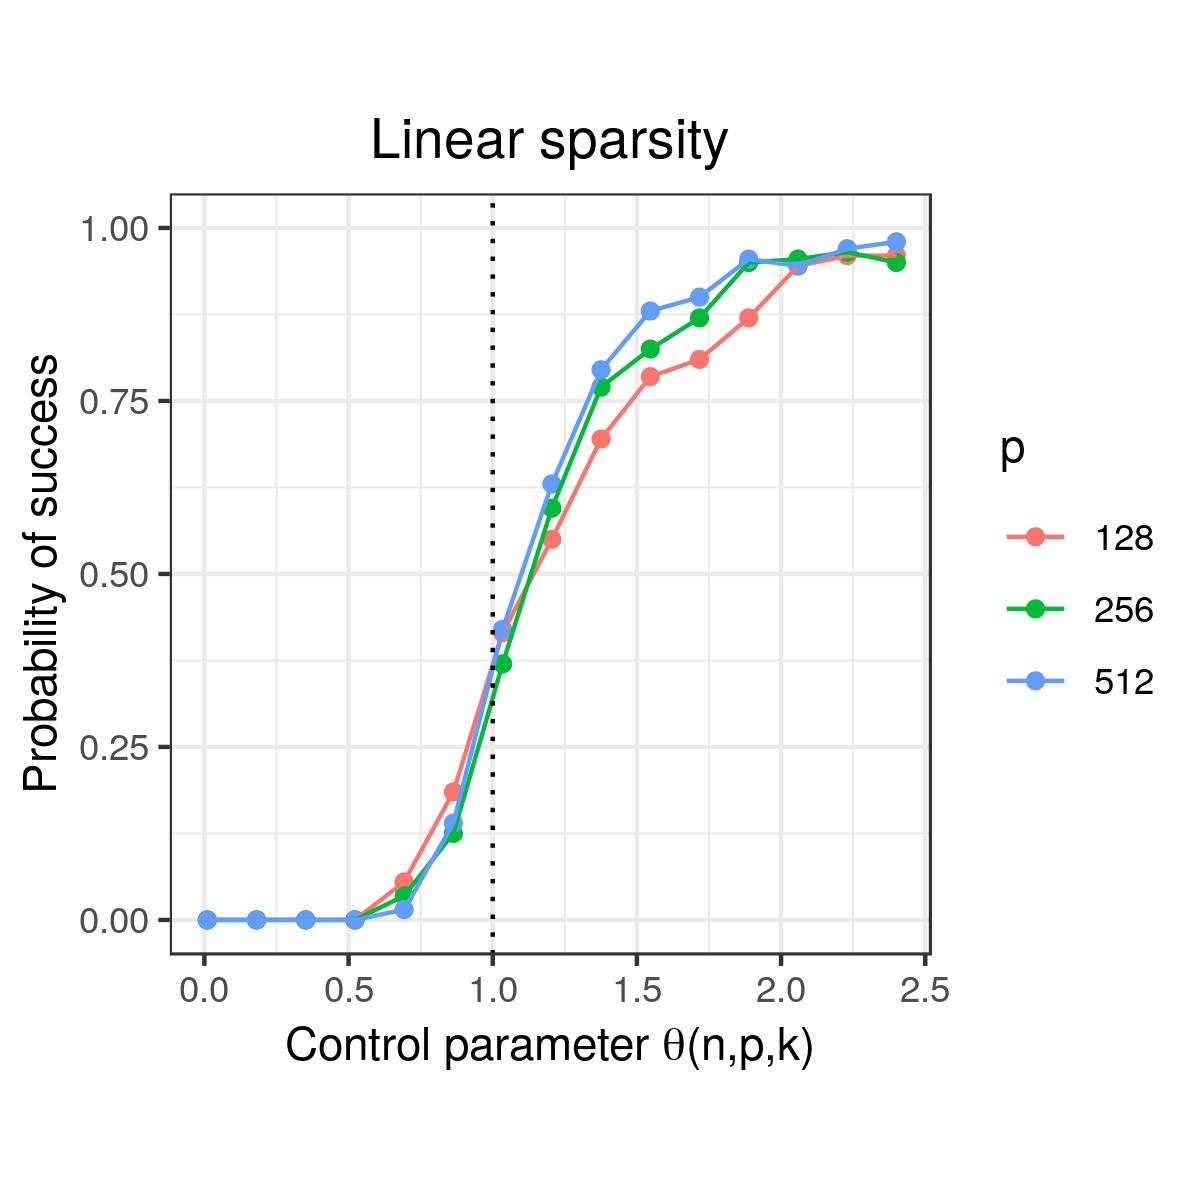
\includegraphics[width=0.9\linewidth]{nonuniform_linear_sparsity_alpha_1}
    \caption{Linear sparsity}
    \label{fig:nonuniform_linear_sparsity_alpha_1}
  \end{subfigure}
  \begin{subfigure}{0.32\textwidth}
    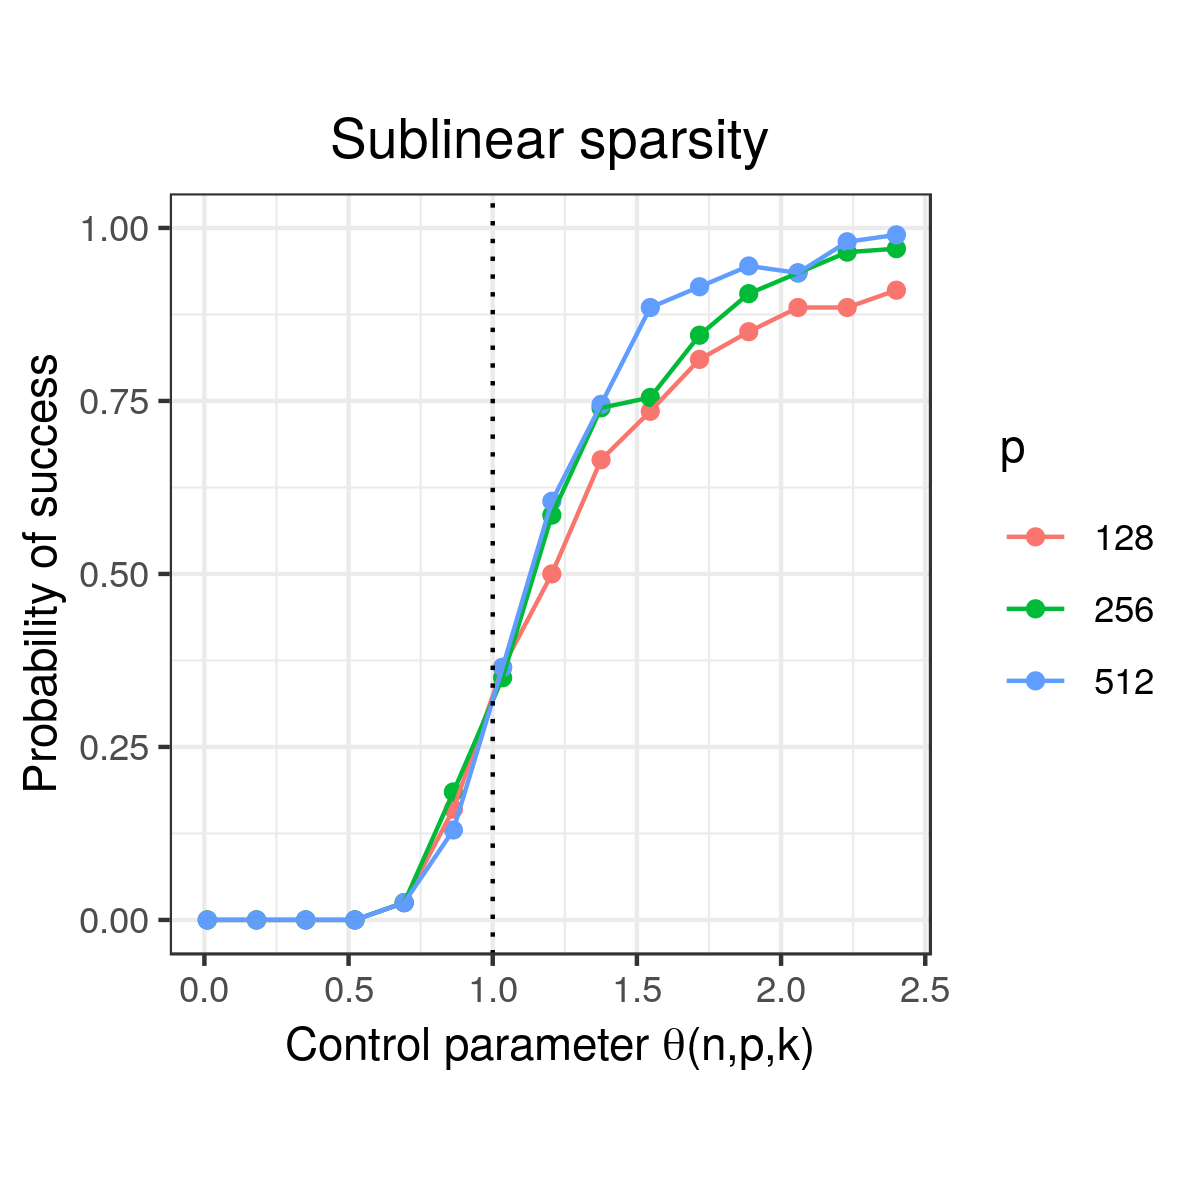
\includegraphics[width=0.9\linewidth]{nonuniform_sublinear_sparsity_alpha_1}
    \caption{Sublinear sparsity}
    \label{fig:nonuniform_sublinear_sparsity_alpha_1}
  \end{subfigure}
  \begin{subfigure}{0.32\textwidth}
    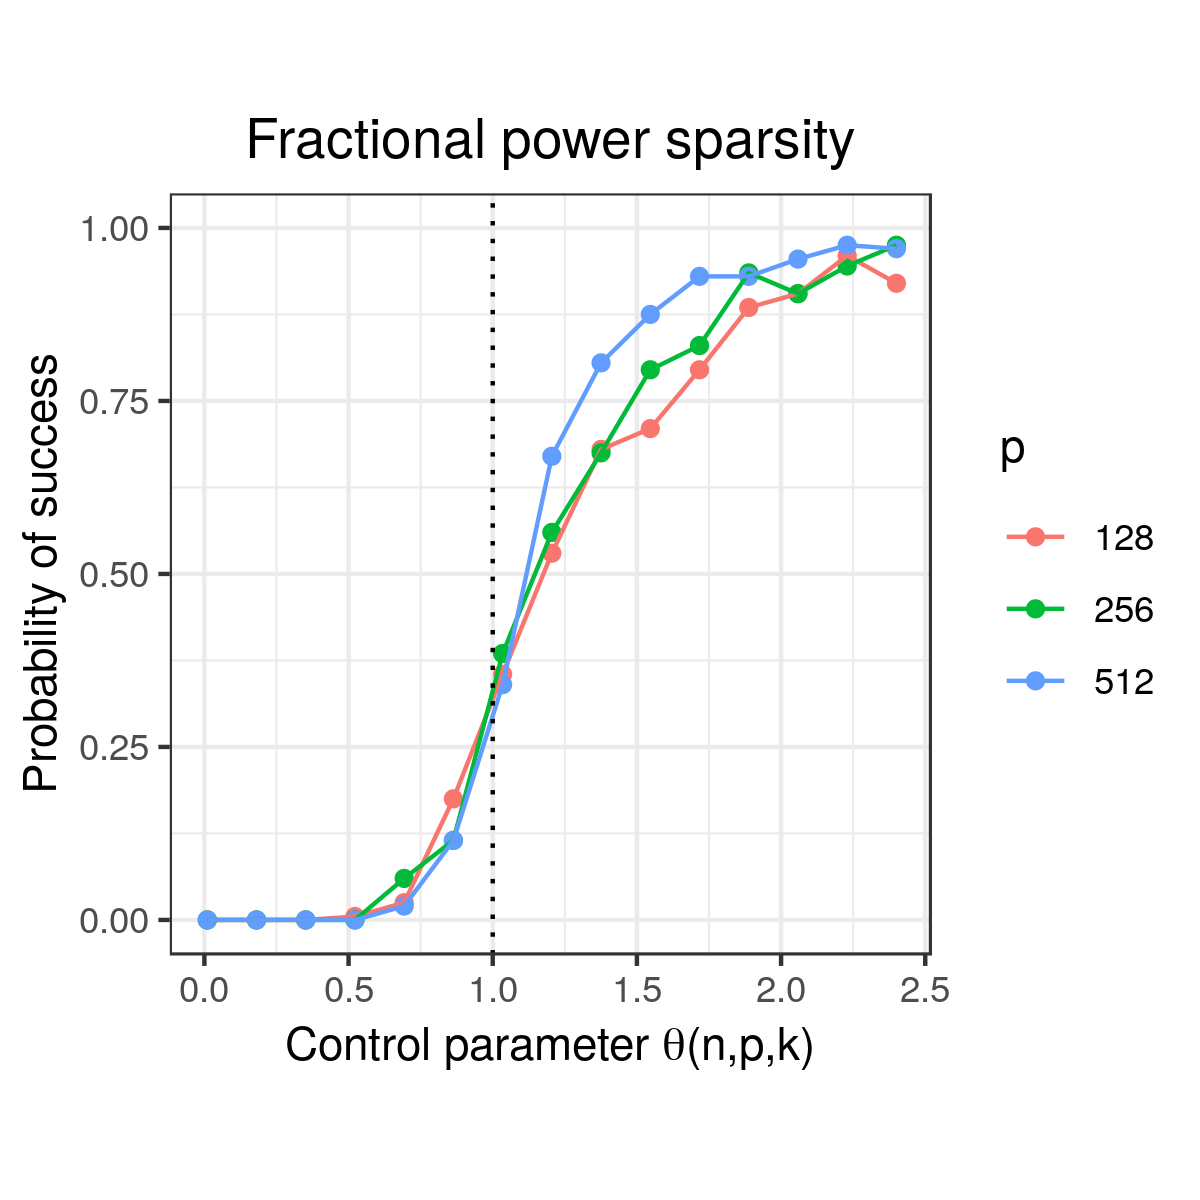
\includegraphics[width=0.9\linewidth]{nonuniform_fractional_power_sparsity_alpha_1}
    \caption{Fractional power sparsity}
    \label{fig:nonuniform_fractional_power_sparsity_alpha_1}
  \end{subfigure}
  \caption{Non-uniform Gaussian ensemble with LASSO}
  \label{fig:nonuniform_alpha_1}
\end{figure}

\subsection*{Custom simulations}

Unlike with the simulations from the paper, the custom simulations
have no theoretical guarantee of incorrect or correct signed support
recovery. Intuitively, since the elastic net penalty is a linear
combination of an $l_1$-penalty and an $l_2$-penalty, we expect the
theoretical results from \cite{wainwright06} to deteriorate as the
contribution of the $l_1$-penalty term is diminished. Specifically, we
consider the results using elastic net mixing parameters of
$\alpha = 0.75$ and $\alpha = 0.50$. The contribution of the
$l_1$-penalty term decreases as $\alpha$ decreases. In particular, the
LASSO corresponds to $\alpha = 1$ (see
\eqref{eq:elastic_net_problem}).

Indeed, the two sets of simulations demonstrate this exact
behavior. In particular, for $\alpha = 0.75$ the estimated probability
of correct signed support recovery is below 1 throughout the range of
control parameters, and \emph{considerably} below 1 for
$\alpha = 0.50$. However, for $\alpha = 0.50$, the elastic net model
performs considerably better under the linear sparsity regime than
under either sublinear or fractional power sparsity. See
Figures~\ref{fig:uniform_alpha_075} and \ref{fig:uniform_alpha_050}.

\begin{figure}[h]
  \centering
  \begin{subfigure}{0.32\textwidth}
    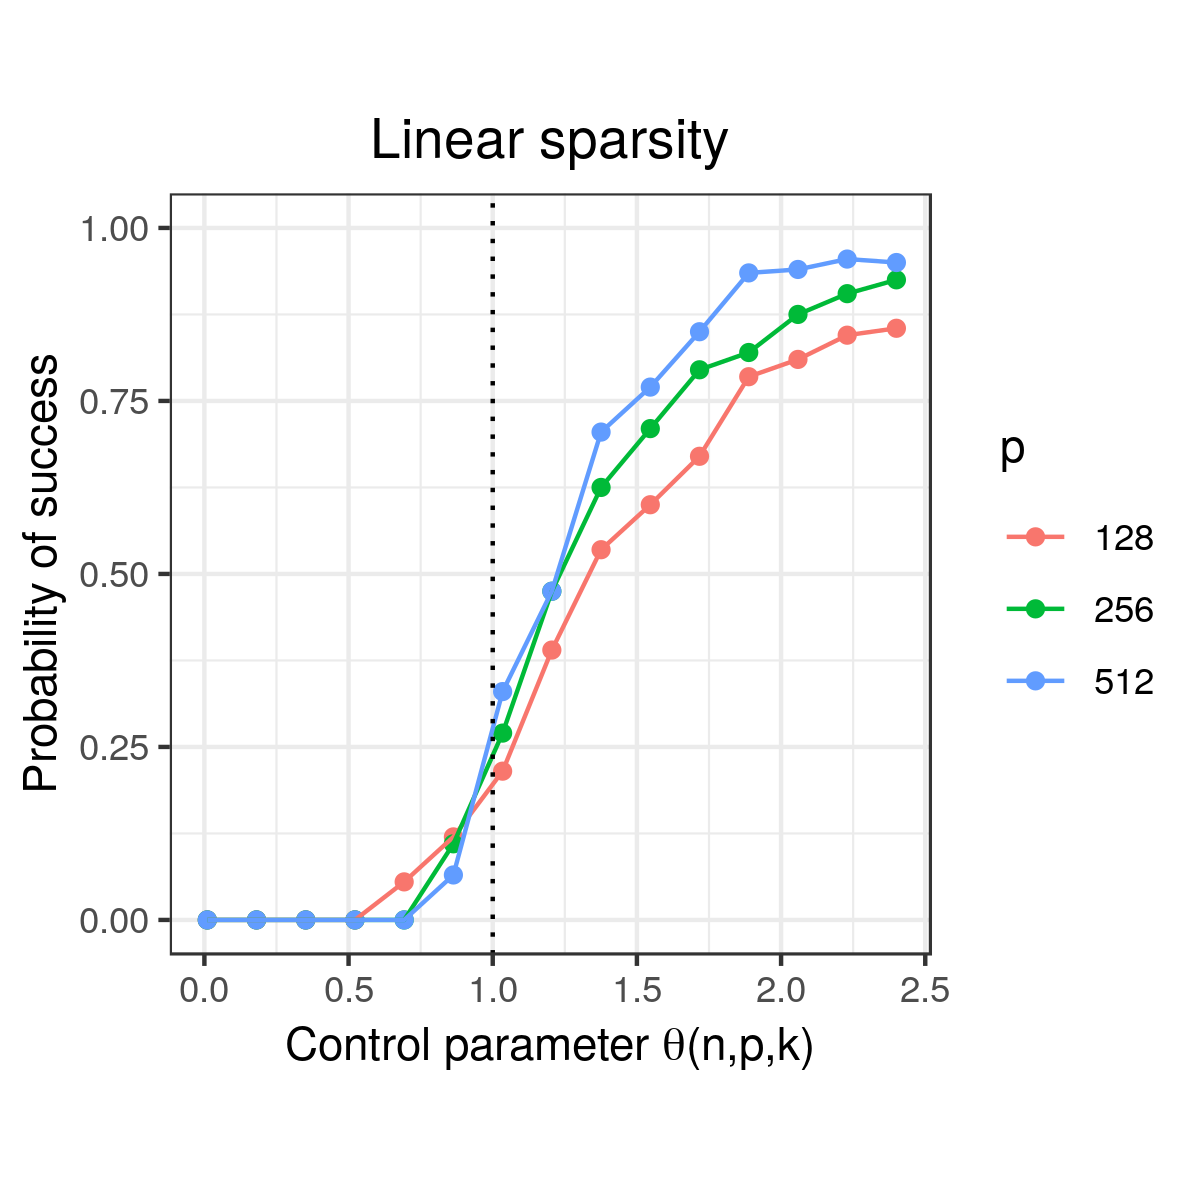
\includegraphics[width=0.9\linewidth]{uniform_linear_sparsity_alpha_075}
    \caption{Linear sparsity}
    \label{fig:uniform_linear_sparsity_alpha_1}
  \end{subfigure}
  \begin{subfigure}{0.32\textwidth}
    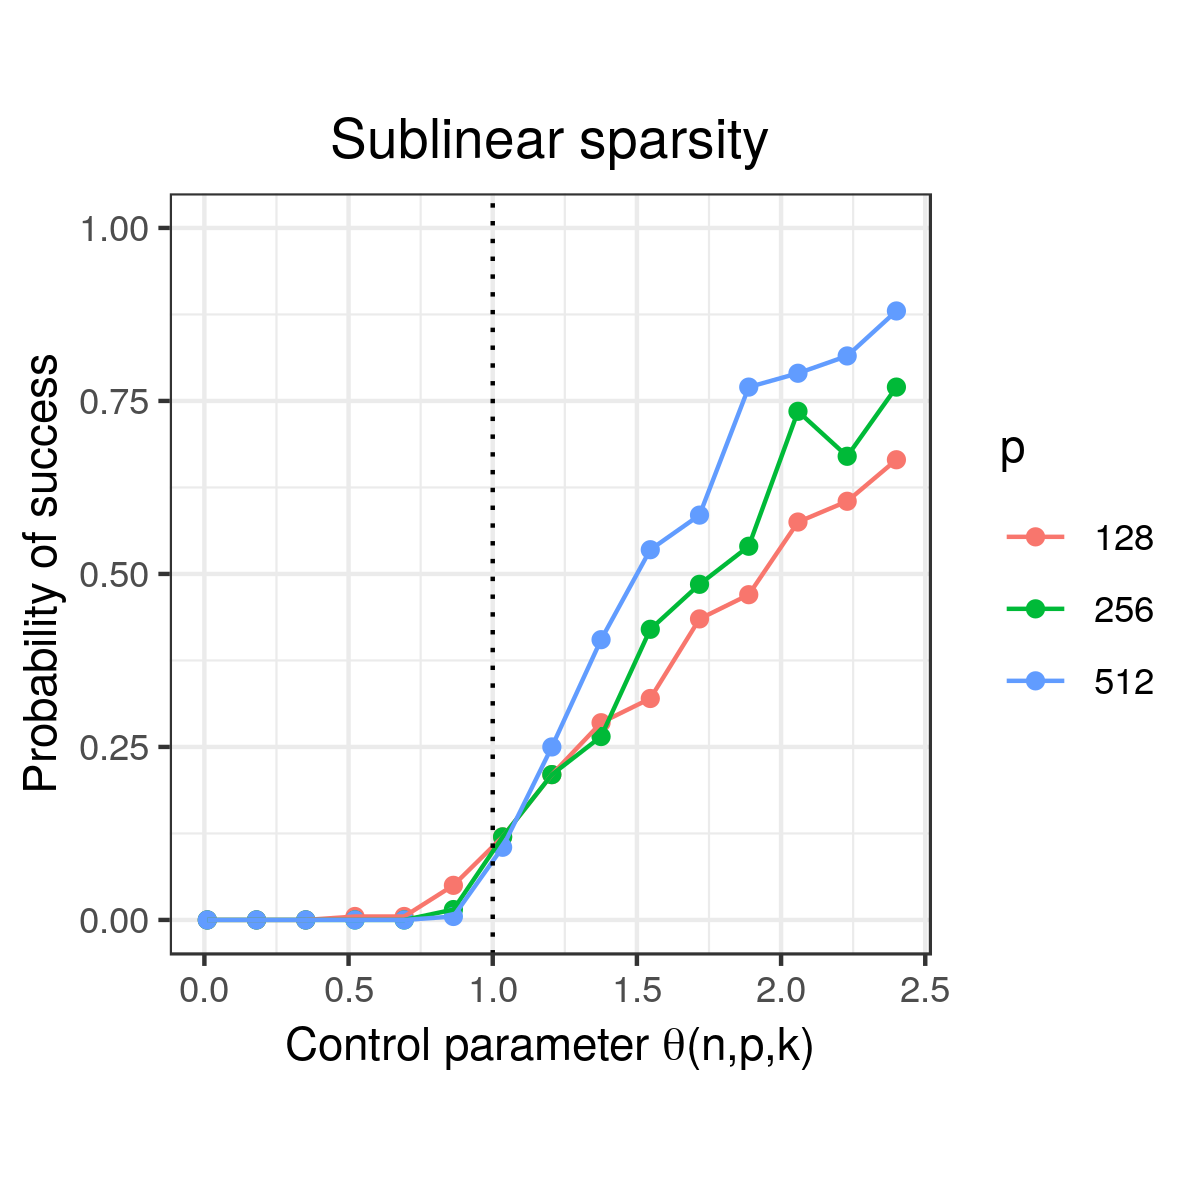
\includegraphics[width=0.9\linewidth]{uniform_sublinear_sparsity_alpha_075}
    \caption{Sublinear sparsity}
    \label{fig:uniform_sublinear_sparsity_alpha_1}
  \end{subfigure}
  \begin{subfigure}{0.32\textwidth}
    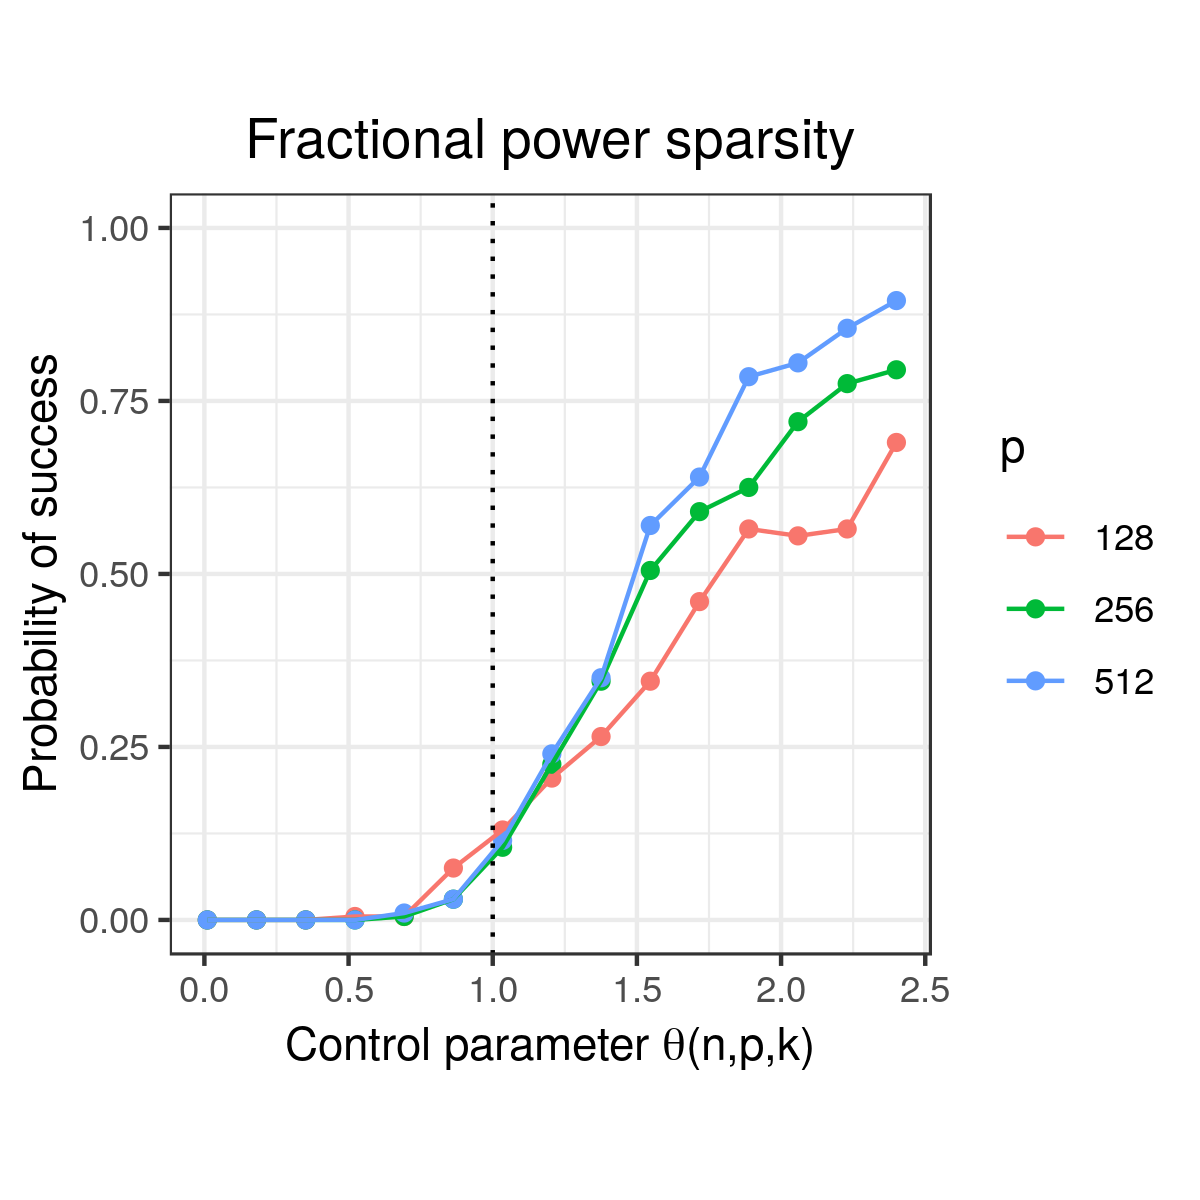
\includegraphics[width=0.9\linewidth]{uniform_fractional_power_sparsity_alpha_075}
    \caption{Fractional power sparsity}
    \label{fig:uniform_fractional_power_sparsity_alpha_1}
  \end{subfigure}
  \caption{Uniform Gaussian ensemble, $\alpha = 0.75$}
  \label{fig:uniform_alpha_075}
\end{figure}

\begin{figure}[h]
  \centering
  \begin{subfigure}{0.32\textwidth}
    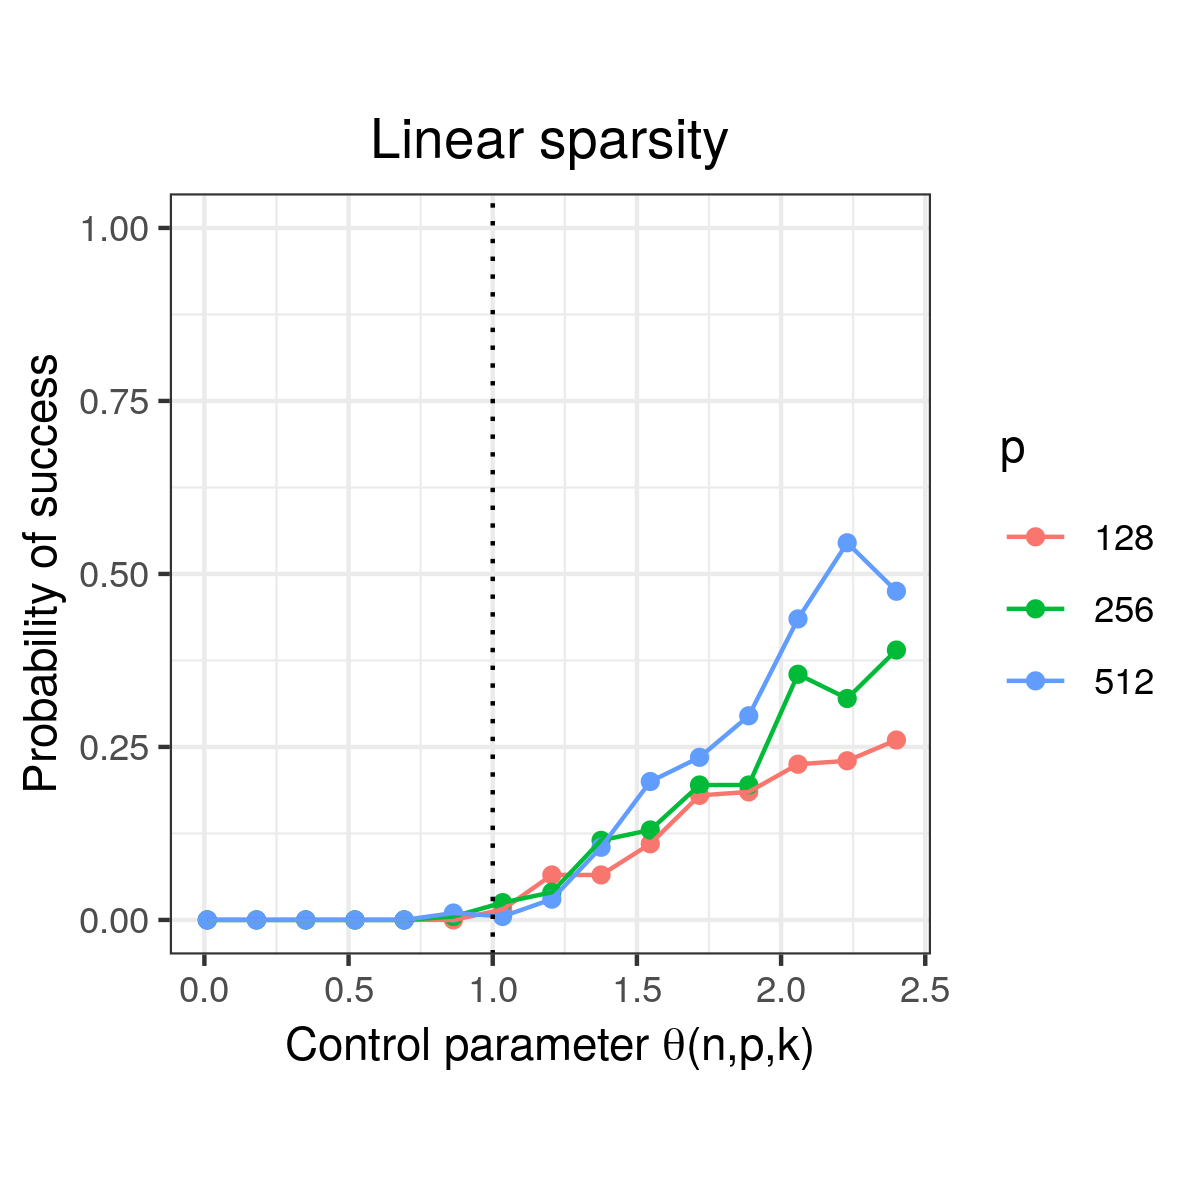
\includegraphics[width=0.9\linewidth]{uniform_linear_sparsity_alpha_050}
    \caption{Linear sparsity}
    \label{fig:uniform_linear_sparsity_alpha_1}
  \end{subfigure}
  \begin{subfigure}{0.32\textwidth}
    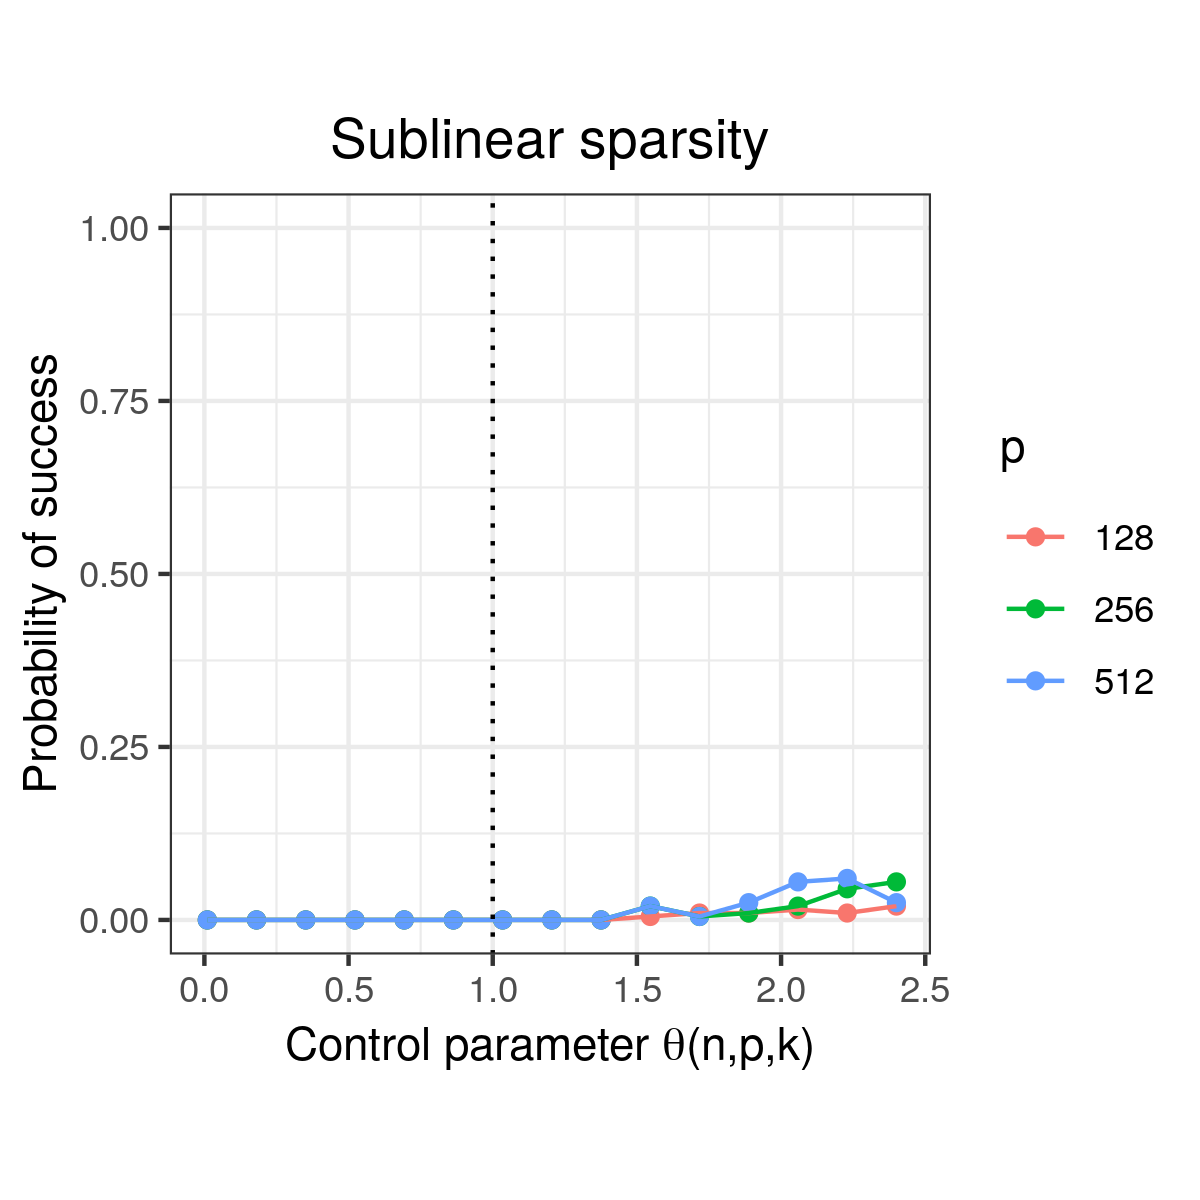
\includegraphics[width=0.9\linewidth]{uniform_sublinear_sparsity_alpha_050}
    \caption{Sublinear sparsity}
    \label{fig:uniform_sublinear_sparsity_alpha_1}
  \end{subfigure}
  \begin{subfigure}{0.32\textwidth}
    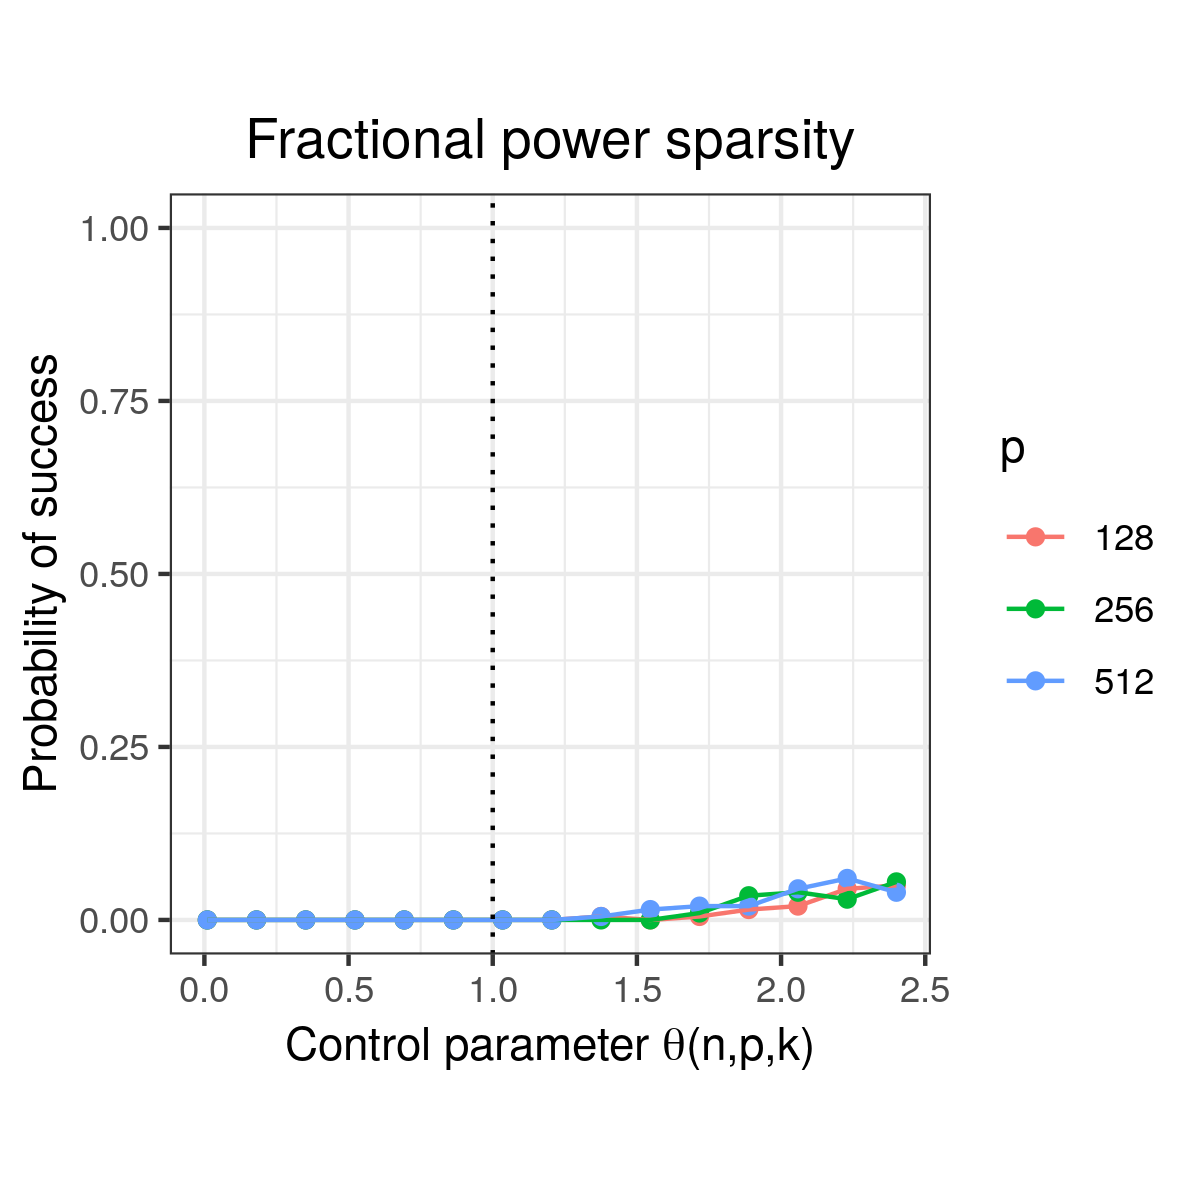
\includegraphics[width=0.9\linewidth]{uniform_fractional_power_sparsity_alpha_050}
    \caption{Fractional power sparsity}
    \label{fig:uniform_fractional_power_sparsity_alpha_1}
  \end{subfigure}
  \caption{Uniform Gaussian ensemble, $\alpha = 0.50$}
  \label{fig:uniform_alpha_050}
\end{figure}

\section*{Conclusion}

This project explored necessary and sufficient conditions for the
LASSO to recover with high probability the true signed support of the
unknown parameter $\beta^\ast$ in the linear model
\eqref{eq:linear_model}. We considered the results concerning signed
support recovery from the paper \cite{wainwright06} in the case of
random design, and reproduced the simulations from this paper in order
to empirically demonstrate these results. Furthermore, we generalized
the simulations from \cite{wainwright06} to the case of elastic net
penalties \cite{zou_hastie05} in the case when the design matrix is
drawn from a uniform Gaussian ensemble. In this case, we have no
theoretical guarantees on the recovery/non-recovery of the true signed
support and, unsurprisingly, these simulations fail to recover the
true signed support with high probability under the conditions
prescribed by \cite{wainwright06}.

\begin{thebibliography}{9}
\bibitem{wainwright06}
  Wainwright, M. (2006).
  \textit{Sharp thresholds for high-dimensional and noisy sparsity
    recovery using $l_1$-constrained quadratic programming (Lasso)}.
  Technical Report 709, Dept. Statistics, Univ. California,
  Berkeley

\bibitem{tibshirani96}
  Tibshirani, R. (1996).
  \textit{Regression shrinkage and selection via the Lasso}.
  J. Roy. Statist. Soc. Ser. B \textbf{58} 267--288

\bibitem{zou_hastie05}
  Zou, H. and Hastie, T. (2005)
  \textit{Regularization and variable selection via the elastic net}.
  J. Roy. Statist. Soc. Ser. B \textbf{67} 301--320

\end{thebibliography}

\end{document}
